\chapter{Solution Design: Improved Kepler Visualisation Tool}\label{C:sd}

This section discusses the deliverable visualisation that will be created as part of this project.
The visualisation for this project will be created using Processing, a Java framework for visualisations. As the time is short for this project, extending a previous visualisation that uses the same dataset, the Kepler Visualisation Tool \cite{kepler_github, kepler_article}, will increase the amount of progress that can be made in the time afforded.

The visualisation was designed to emphasis small multiples and filtering of the Exoplanets to display the information more clearly to users. 
\\\\
Instead of the visualisation only answering the 5 key questions as proposed in the proposal, the aim will now be displaying as much of the information in the dataset as possible without detracting from the effectiveness of the visualisation whilst still answering the questions. 
\\\\
This is because the 5 questions did not fully utilize the information in the dataset. 

However I will need to ensure the effectiveness of the visualisation does not become diminished by trying to convey to much information which would lead to cluttering and overlapping in the visualisation, as well as information overload for users. There will also be larger emphasis placed on making the existing system more usable by improving the interaction methods for users. The following list outlines the new requirements for the visualisation being developed. This will be done by 
providing GUI elements for each form of interaction with the system, as well as ensuring all interaction methods are intuitive for users. 
\subsection{Visualisation Layout}
\subsubsection{Component Layout}
As the majority of the interaction and movement of visualisation elements occurs in the center of the window it caused a aspect ratio that SOMETHING SOMETHING. It was BETTER to use 2 vertical columns to view and control the visualisation as it had a higher aspect ratio which allowed more of the content to be seen on the screen at once thanks to the fact that the majority of computer screens have a wide ratio.

\begin{figure}[h!]
  \centering
      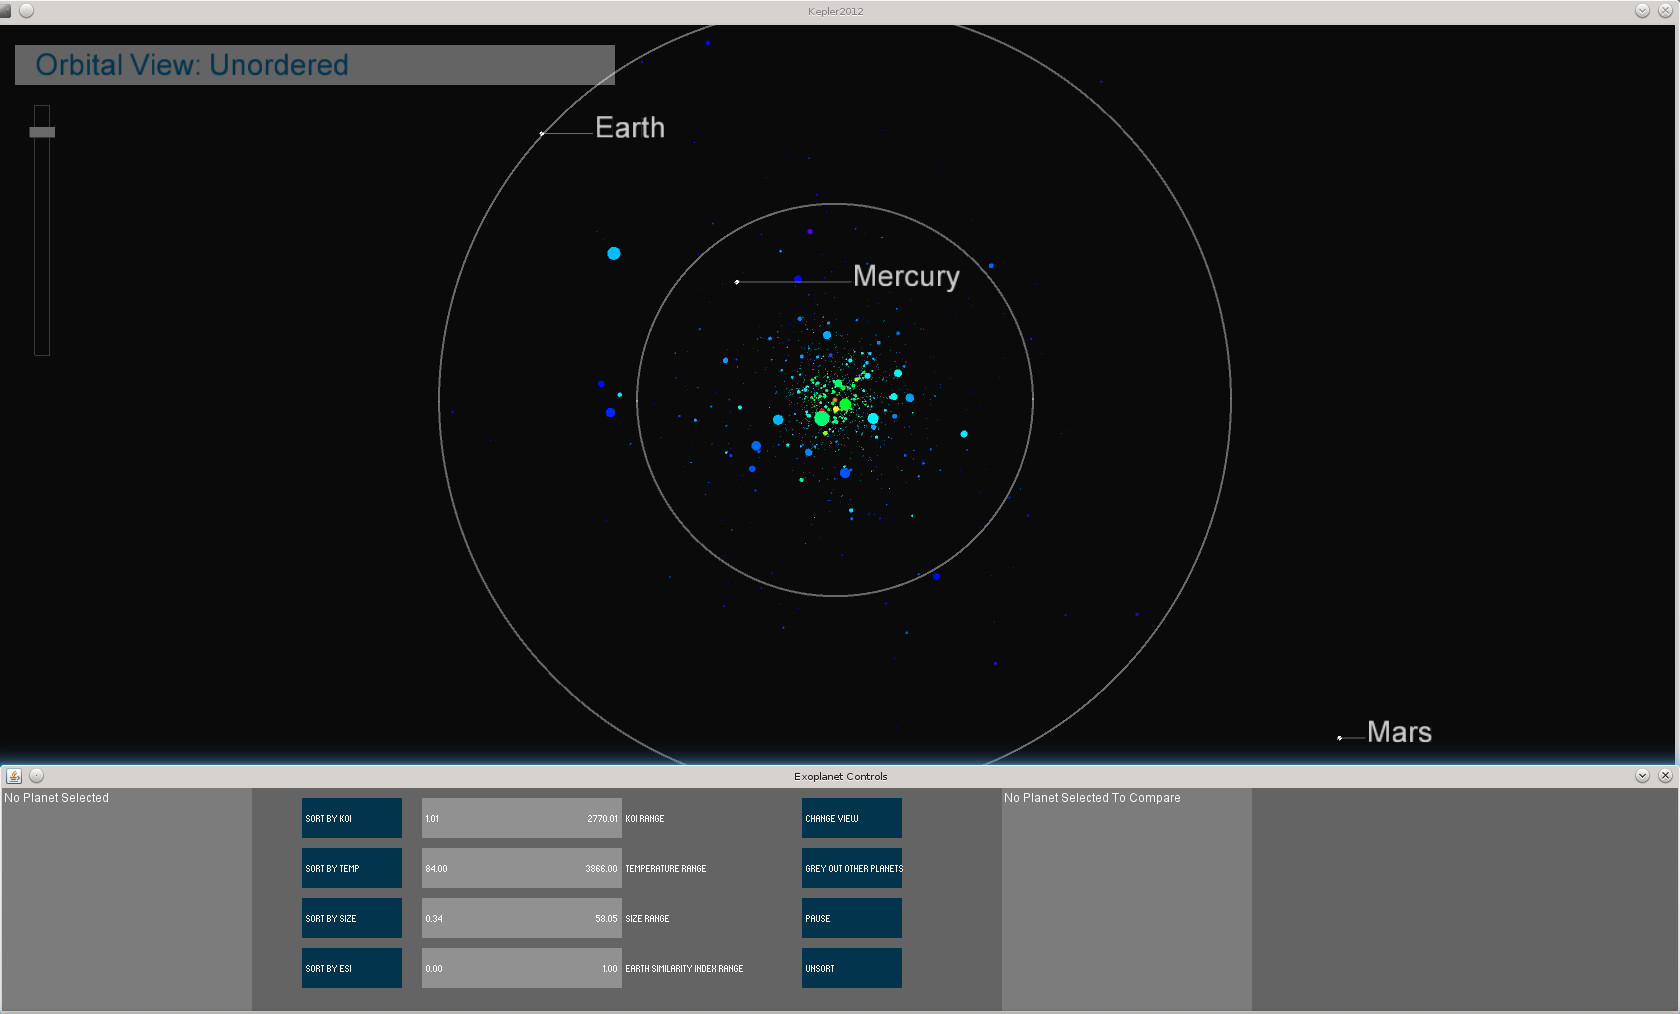
\includegraphics[width=0.8\textwidth]{images/layout_horizontal.jpg}
  \caption{Original Horizontal Layout}  
        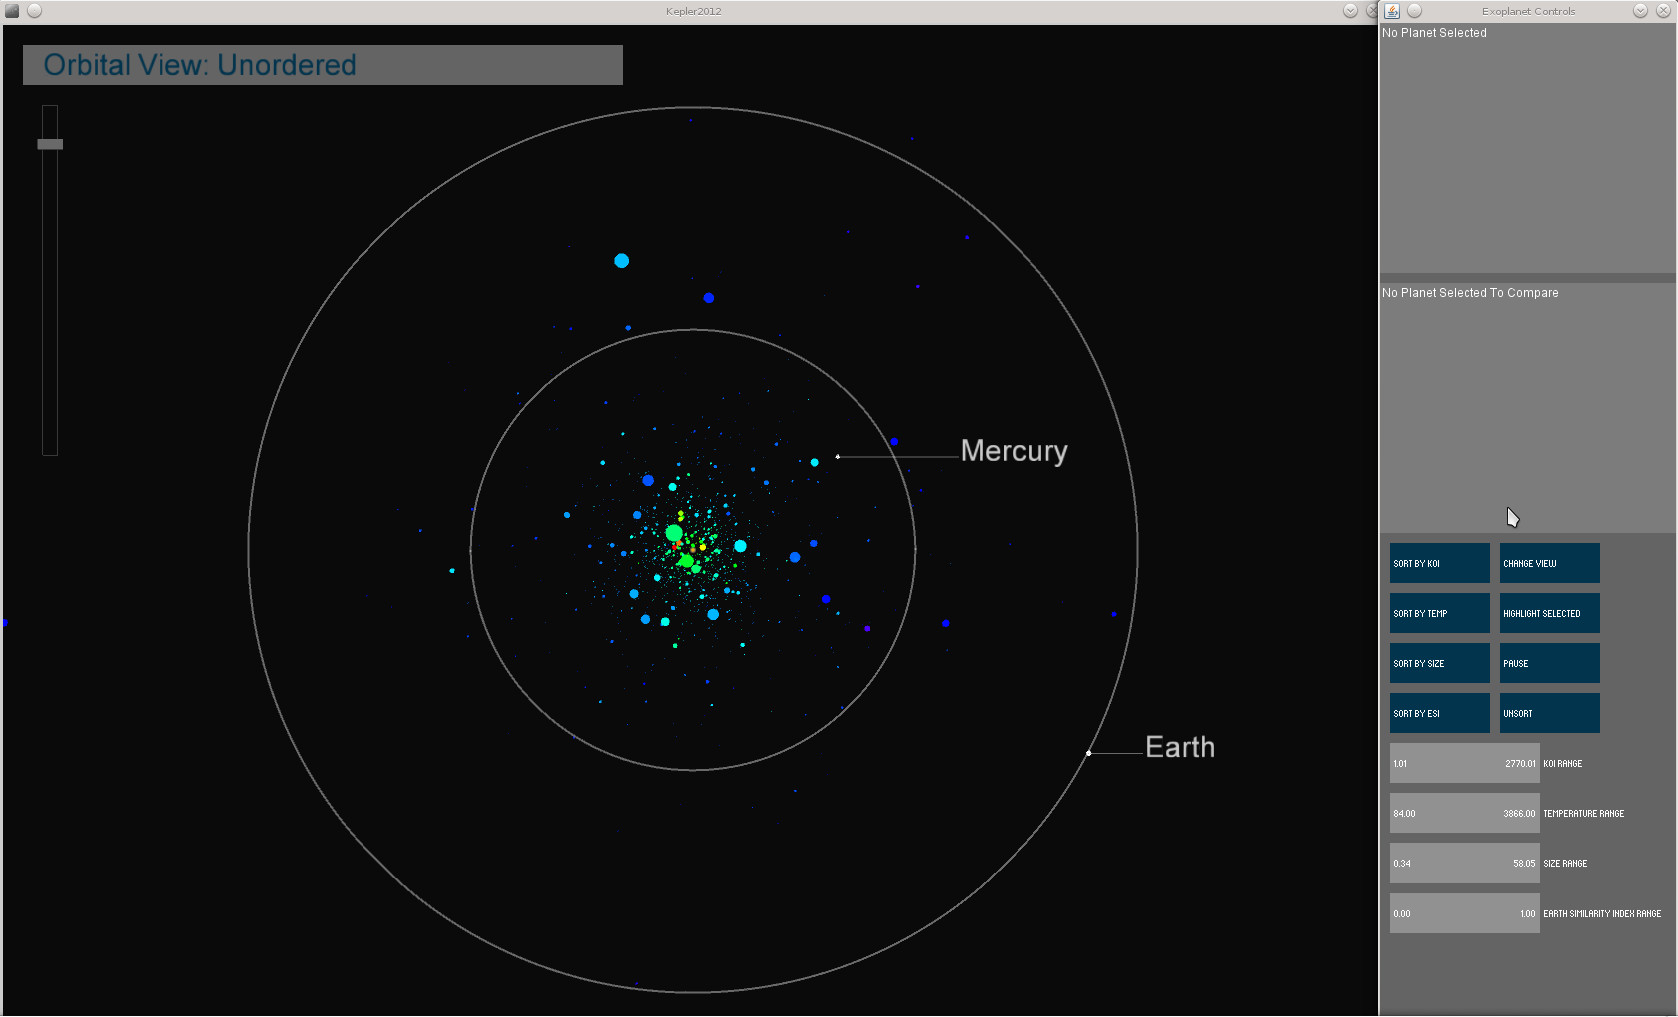
\includegraphics[width=0.8\textwidth]{images/layout_vertical.jpg}
  \caption{Improved Vertical Layout}
\end{figure}

Selection of planets
\section{Extensions from project initiation document}
Kinect for improved user interaction and immersion
